\documentclass[reprint,english,notitlepage,nofootinbib]{revtex4-1}  %

\usepackage{silence}
\WarningFilter{revtex4-1}{Repair the float}
 
\usepackage[utf8]{inputenc}
\usepackage[english]{babel}
\usepackage{physics,amssymb} 
\usepackage{graphicx}        
\usepackage{xcolor}          
\usepackage{hyperref}        
\usepackage{tikz, pgfplots}
\usepackage{listofitems}
\usepackage{listings}
\usepackage{csquotes}
%\usepackage{subfigure}  
\usepackage{here}
\usepackage{fancyvrb}
\usepackage{fontawesome}
\usepackage{fontspec}
\usepackage{algorithm}
\usepackage{algorithmic}
\usepackage{subcaption}
\bibliographystyle{plain}
\hypersetup{ % this is just my personal choice, feel free to change things
    colorlinks,
    linkcolor={red!50!black},
    citecolor={blue!50!black},
    urlcolor={blue!80!black}}

%% Defines the style of the programming listing
%% This is actually my personal template, go ahead and change stuff if you want
\lstset{ %
	inputpath=,
	backgroundcolor=\color{white!88!black},
	basicstyle={\ttfamily\scriptsize},
	commentstyle=\color{magenta},
	language=Python,
	morekeywords={True,False},
	tabsize=4,
	stringstyle=\color{green!55!black},
	frame=single,
	keywordstyle=\color{blue},
	showstringspaces=false,
	columns=fullflexible,
	keepspaces=true}

 %% TiKz stuff
\usetikzlibrary{positioning,chains}
\colorlet{myred}{red!80!black}
\colorlet{myblue}{blue!80!black}
\colorlet{mygreen}{green!60!black}
\colorlet{myorange}{orange!70!red!60!black}
\colorlet{mydarkred}{red!30!black}
\colorlet{mydarkblue}{blue!40!black}
\colorlet{mydarkgreen}{green!30!black}

\definecolor{mako1}{HTML}{38aaac}
\definecolor{mako2}{HTML}{357ba3}
\definecolor{mako3}{HTML}{40498e}

% STYLES
\tikzset{
  >=latex, % for default LaTeX arrow head
  node/.style={thick,circle,draw=mako1,minimum size=22,inner sep=0.5,outer sep=0.6},
  node in/.style={node,black,draw=mako1!30!black,fill=mako1!40},
  node hidden/.style={node,black,draw=mako2!30!black,fill=mako2!40},
  node out/.style={node,black,draw=mako3!30!black,fill=mako3!40},
  connect/.style={->,thick,mako3!40!black}, %,line cap=round
  connect arrow/.style={-{Latex[length=4,width=3.5]},thick,mako3!40!black,shorten <=0.5,shorten >=1},
  node 1/.style={node in}, % node styles, numbered for easy mapping with \nstyle
  node 2/.style={node hidden},
  node 3/.style={node out}
}
\def\nstyle{int(\lay<\Nnodlen?min(2,\lay):3)}


\begin{document}

%==========================================================
%------------------ Project content -----------------------
%==========================================================

%------------------ Title ---------------------------------
\title{Project 2}
\author{Even Sletteng Garvang, Ellen-Beate Tysvær, Janita Ovidie Sandtrøen Willumsen \\ \faGithub \, \url{https://github.com/jovidie/FYS-STK4155-Project-2}}        
\date{\today}
\noaffiliation

%================================================================
%------------------------- Abstract -----------------------------
%================================================================
% You summarize your work short and sweet, and reveal very sensible findings. Good! For an abstract, it is customary to include some stage setting at the beginning. The first sentence should reveal what field we are in. The next few might narrow in on which specific subfield we are in. Then, you explain your motivation, or present the "gap" in knowledge that your research will fill.

% Of course, it's not easy to make a motivation for this project, because it is just a project! But I encourage you to attempt to create a motivation that corresponds to the results you want to highlight here. For example, maybe you see a need to explore when to use OLS versus Ridge, because OLS performs better than Ridge unless there's overfitting. It's up to you :) 


% The abstract can then conclude with the broader impact of your findings. What does it mean for the scientific community? Or the general public?
\begin{abstract}
    Abstract
\end{abstract}
\maketitle

%------------------ Body ----------------------------------
%\mainmatter
%================================================================
\section{Introduction}\label{sec:introduction}
% Motivate the reader and present overarching ideas, and 
% background on the subject of the project. Mention what I have 
% done and present the structure of the report, that is how it is 
% organized.
%================================================================


The applications of artificial intelligence (AI) are many-faceted and a hot topic in most fields
of industry and science today. Although the concept of AI is old, it has recently regained popularity during the current AI boom, 
which began in 2010 by a combination of advances in the field of deep learning. 

Deep learning is a sub-category of machine learning that uses 
artificial neural networks to make informed decisions about a dataset. These artificial neural networks (ANN) get their name from 
the process which they are thought to simulate; neurons in the brain that communicate through a shared network. 

The concept of machine intelligence was presented for the first time when Turing presented his idea of 
a Turing machine in 1936 \cite{turing_36}, a machine that was supposed to mimic human intelligence. However the actual idea of brain mimicry and ANN's is considered to first be proposed by McCullough and Pitts in 1943 \cite{mccu_pitt}.

More about the use of ANN on cancer ...

In this project, we create an artificial neural network from scratch, as well as a model for logistic regression and a set of optimizers 
in order to explore how our ANN compares to simpler logistic regression models. We also explore how our ANN compares to previously 
explored linear regression methods from Project 1. Finally, we use our ANN on the Wisconsin Breast Cancer Dataset to predict if a
tumor is bening or malignant. 

We found that ...


%==============================================================
\section{Methods}\label{sec:methods}
% Describe the methods and algorithms used, include any formulas. 
% Explain how everything is implemented, and possibly mention the structure of the algorithm. 
% Add demonstrations such as tests, selected runs and validations. 
%==============================================================
Janita, Even writes about GD and SGD?
%------------ Background? -------------------------------------
\subsection{Regression vs. Classification}\label{ssec:regression_classification}


%------------ Logistic Regression -----------------------------
\subsection{Logistic Regression}\label{ssec:logreg}
Logistic regression is a method of classification, which estimates the probability of being in a certain class. In contrast to linear regression methods, where the outcome is continuous function, the outcome of logistic regression is a linear classifier which gives a decision boundary between classes. This method is often used as a baseline model, particularly in problems in the nature of binary classification, which is what we will focus on.

The sigmoid function is used to fit the model, and is written as
\begin{equation}\label{eq:sigmoid}
    p(z) = \frac{1}{1 + \exp{-z}} , 
\end{equation}
where $z$ is the model's prediction. We define the cost function as the log-likelihood in Equation \eqref{eq:log_likelihood}, which is derived from the Maximum Likelihood Principle.
\begin{equation}\label{eq:log_likelihood}
    \mathcal{C}(\mathbf{\beta}) = - \sum_{i=1}^{n} (y_{i} (\beta_{0} + \beta_{1} x_{i}) - \log (1 + \exp{\beta_{0} + \beta_{1} x_{i}})))
\end{equation}


%------------ Gradient Descent --------------------------------
\subsection{Gradient Descent}\label{ssec:gradient_descent}

%% work-in-progress her, må samle tankene for å forklare dette på en god måte!
For both regression and classification, we want to optimize a set of parameters $\theta$ given a cost function $C(X, \theta)$. This is ususally done by minimizing the cost function. One way of finding the minimum of the cost function given our parameters is by gradient descent (Algorithm \ref{alg:gd}). In gradient descent you start with a random set of parameters, and change these in small steps towards the optimal values by moving iteratively along a gradient \cite{Goodfellow:2016:deep_learning}. The step size is determined by the hyperparameter $\eta$, and is also called the learning rate. The gradient is found by calculating the first derivatives of the cost function with respect to the parameters, and evaluating these for each iteration. The algorithm is run either until some convergence criterion is reached (e.g., gradients approaching 0) it reaches the maximum number of iterations.

While gradient descent effectively minimizes the cost function given the starting parameters, the algorithm can find a local minimum, rather than the lower global minimum. To avoid that the algorithm gets stuck in local minima, it is common to use a small random subset of your data each time you compute the gradients, rather than the full data. This method is known as stochastic gradient descent (Algorithm \ref{alg:sgd}).

\begin{algorithm}
\caption{Gradient descent}\label{alg:gd}
\begin{algorithmic}[1]
    \STATE Initialize parameters $\theta = \theta_0$
    \STATE Choose a learning rate $\eta > 0$
    \REPEAT
        \STATE Compute the gradient $\nabla C(\theta)$
        \STATE Update the parameters: $\theta \leftarrow \theta - \eta \nabla C(\theta)$
    \UNTIL{convergence}
\end{algorithmic}
\end{algorithm}

\begin{algorithm}
\caption{Stochastic gradient descent with mini-batches}\label{alg:sgd}
\begin{algorithmic}[1]
    \STATE Initialize parameters $\theta = \theta_0$
    \STATE Choose a learning rate $\eta > 0$
    \STATE Choose mini-batch size $m$
    \STATE Set number of epochs $K$
    \FOR{epoch $= 1$ to $K$}
        \STATE Shuffle the training data
        \FOR{each mini-batch \( \mathcal{B}_i \) of size $m$}
            \STATE Compute the gradient: $\nabla_{\mathcal{B}_i} C(\theta)$
            \STATE Update the parameters: $\theta \leftarrow \theta - \eta \nabla_{\mathcal{B}_i} C(\theta)$
        \ENDFOR
    \ENDFOR
\end{algorithmic}
\end{algorithm}

%------------ Feed-Forward Neural Network ---------------------
\subsection{Feed-Forward Neural Network}\label{ssec:ffnn}
In recent years, neural networks have shown promise in solving both regression and classification problems. They and have evolved into several types of networks, with the simplest one called feed-forward neural network (FFNN). In FFNNs, information moves through the layers in one direction, and the network is said to be fully connected if each neuron in a layer is connected to all neurons in the next layer, illustrated in Figure \ref{fig:ffnn}. 

\begin{figure}[h!]
    \centering
    \resizebox{0.9\linewidth}{!}
    {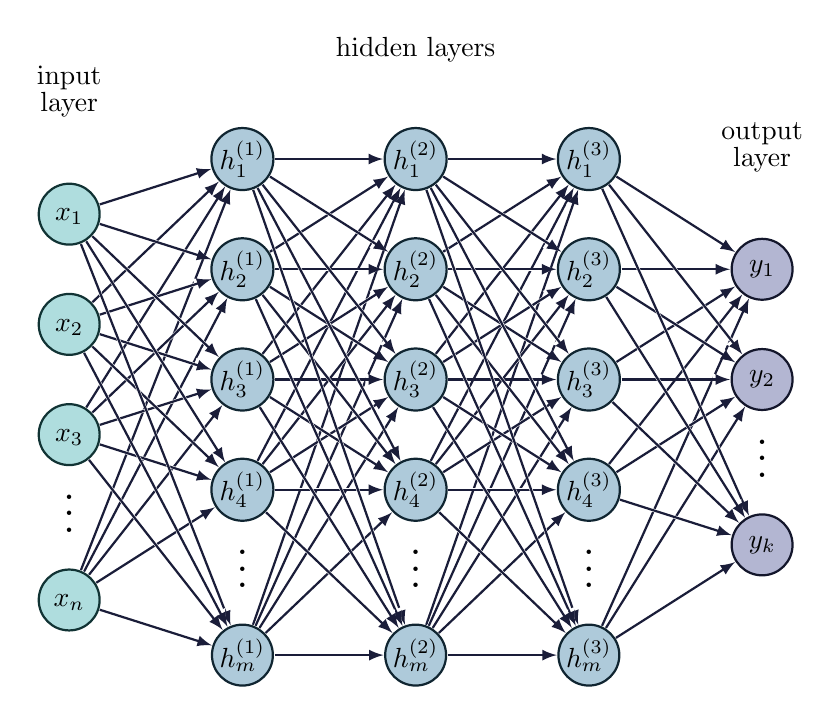
\begin{tikzpicture}[x=2.2cm,y=1.4cm]
      \readlist\Nnod{4,5,5,5,3}
      \readlist\Nstr{n,m,m,m,k}
      \readlist\Cstr{\strut x,h^{(\prev)},h^{(\prev)},h^{(\prev)},y} 
      \def\yshift{0.5} 
      % \message{^^J  Layer}
      \foreachitem \N \in \Nnod{ % loop over layers
        \def\lay{\Ncnt} % alias of index of current layer
        \pgfmathsetmacro\prev{int(\Ncnt-1)} % number of previous layer
        \message{\lay,}
        \foreach \i [evaluate={\c=int(\i==\N); \y=\N/2-\i-\c*\yshift;
                     \index=(\i<\N?int(\i):"\Nstr[\lay]");
                     \x=\lay; \n=\nstyle;}] in {1,...,\N}{ % loop over nodes
          % NODES
          \node[node \n] (N\lay-\i) at (\x,\y) {$\Cstr[\lay]_{\index}$};
          
          % CONNECTIONS
          \ifnum\lay>1 % connect to previous layer
            \foreach \j in {1,...,\Nnod[\prev]}{ % loop over nodes in previous layer
              \draw[connect,white,line width=1.2] (N\prev-\j) -- (N\lay-\i);
              \draw[->,connect] (N\prev-\j) -- (N\lay-\i);
              %\draw[connect] (N\prev-\j.0) -- (N\lay-\i.180); % connect to left
            }
          \fi % else: nothing to connect first layer
          
        }
        \path (N\lay-\N) --++ (0,1+\yshift) node[midway,scale=1.5] {$\vdots$};
      }
      
      % LABELS
      \node[above=0.5,align=center,black] at (N1-1.90) {input\\[-0.2em]layer};
      \node[above=0.5,align=center,black] at (N3-1.90) {hidden layers};
      \node[above=0.5,align=center,black] at (N\Nnodlen-1.90) {output\\[-0.2em]layer};
    \end{tikzpicture}}
    %\includegraphics[width=0.5\linewidth]{}
    \caption{Illustration of a feed-forward neural network with one input layer, three hidden layers, and one output layer, where $n$, $m$ and $k$ indicate the number of neurons in the respective layer.}
    \label{fig:ffnn}
\end{figure}
The architecture of a neural network is often determined by the problem to be solved. According to the universal approximation theorem, a FFNN with a minimum of one input layer, one hidden layer with a non-linear activation function, and one linear output layer, is sufficient to approximate a continuous function \cite[194]{Goodfellow:2016:deep_learning}. 

The output of a hidden layer can be written as 
\begin{equation}\label{eq:ffnn}
    \mathbf{h} = a \Big( \mathbf{W}^{T} \mathbf{x} + \mathbf{b} \Big) ,
\end{equation}
where $a$ is a non-linear activation function, $\mathbf{W}$ is the weight matrix, $\mathbf{x}$ is input, and $\mathbf{b}$ is the bias. 

\subsubsection{Weights and biases}\label{sssec:weights_biases}
The technique used to initialize the weights and biases in the FFNN can be vital for how fast the network learns. For a less ideal method, the network may need more iterations to find an optimal solution. Whereas a clever initialization may reduce the number of iteration needed, as the weight are some of the hyper-parameters that needs tuning. 

\subsubsection{Activation functions}\label{sssec:activation_functions}


\subsubsection{Cost functions}\label{sssec:cost_functions}


\subsubsection{Forward propagation}\label{sssec:forward_propagation}


\subsubsection{Back-propagation}\label{sssec:backpropagation}


%------------ Data --------------------------------------------
\subsection{Data}\label{ssec:data}


%------------ Tools -------------------------------------------
\subsection{Tools}\label{ssec:tools}
The models were implemented in \verb|Python|, and the figures produced using the \verb|matplotlib| library, and stylized using \verb|seaborn|.
%================================================================
\section{Results}\label{sec:results}
% Present results and give a critical discussion of my work in 
% the context of other work. Relate the work to previous studies, 
% and make sure the results are reproducible. Include information 
% in figure captions such that they can give the reader enough to 
% understand the main gist of the report.
%================================================================

Future works: 
- Dropout rate to prevent overfitting
- 
%================================================================
\section{Conclusion}\label{sec:conclusion}
% State main findings and interpretations, and try to present 
% perspectives for future work. Discuss pros and cons of methodd, 
% and possible improvements.
%================================================================
\newpage

 
%------------------ Bibliography --------------------------
\onecolumngrid
\newpage 
% \nocite{*}
\bibliography{references}

%------------------ Appendix ------------------------------
\newpage
\twocolumngrid
%================================================================
\appendix
% Additional calculations used to validate the codes, these 
% selected calculations can be listed with few comments. Can also 
% include listing of the code if you feel this is necessary
%================================================================

%------------------ Structure -----------------------------
% \tableofcontents 

%==========================================================
%------------------ End of project content ----------------
%==========================================================
\end{document}